\documentclass[11pt]{article}

\usepackage[letterpaper,top=1in,bottom=1in,left=1.25in,right=1.25in]{geometry}
\usepackage{setspace}
\usepackage[parfill]{parskip}
\usepackage{hyperref}
\usepackage{enumitem}
\usepackage{tikz,ifthen,xstring,calc,pgfkeys,pgfopts}
\usepackage{tikz-uml}
\usepackage{float}

\tikzumlset{fill class=black!15}

\begin{document}

\begin{figure}

  \begin{center}
    \begin{tikzpicture}
      
      \umlclass[x=2, y=0, width=15ex]{TetrisPiece}{
        current\_block\_locations: vector$<$unique\_ptr$<$Point$>>$
      }{
        rotate() : void \\
        get\_rotated\_block\_locations() : vector$<$unique\_ptr$<$Point$>>$\& \\
        get\_block\_locations() : vector$<$unique\_ptr$<$Point$>>$\& \\
        fall() : void \\
        shift( direction\_unit: int ) : void \\
        \umlvirt{original\_block\_locations() : vector$<$unique\_ptr$<$Point$>>$}
      }
      
      \umlemptyclass[x=-4, y=-7, width=15ex]{BarPiece}
      \umlemptyclass[x=0, y=-7, width=15ex]{BlockPiece}
      \umlemptyclass[x=4, y=-7, width=15ex]{EssPiece}
      \umlemptyclass[x=8, y=-7, width=15ex]{ZeePiece}      
      \umlemptyclass[x=-2, y=-10, width=15ex]{EllPiece}
      \umlemptyclass[x=2, y=-10, width=15ex]{JayPiece}
      \umlemptyclass[x=6, y=-10, width=15ex]{TeePiece}

      \umlinherit[geometry=|-|]{BarPiece}{TetrisPiece}
      \umlinherit[geometry=|-|]{BlockPiece}{TetrisPiece}
      \umlinherit[geometry=|-|]{EssPiece}{TetrisPiece}
      \umlinherit[geometry=|-|]{ZeePiece}{TetrisPiece}
      \umlinherit[geometry=|-|]{JayPiece}{TetrisPiece}

      \umlVHVinherit[arm1=6.5cm]{EllPiece}{TetrisPiece}
      \umlVHVinherit[arm1=6.5cm]{TeePiece}{TetrisPiece}

    \end{tikzpicture}
  \end{center}

  \caption{TetrisPiece architecture}

\end{figure}

\begin{figure}

  \begin{center}
    
\begin{tikzpicture}
      
      \umlclass[x=-6, y=0, width=15ex]{TetrisComponentFactory}{
      }{
        build\_component( piece\_type : PieceType ) : unique\_ptr$<$TetrisPiece$>$
      }
      
      \umlemptyclass[x=2, y=0, width=15ex]{TetrisPiece}

      \umldep{TetrisComponentFactory}{TetrisPiece}

    \end{tikzpicture}
  \end{center}

  \caption{TetrisComponentFactory architecture}

\end{figure}

\end{document}
